\section{Results}
\subsection{No stabilisation}
\begin{frame}{No stabilisation}
    \begin{center}
\includemedia[
    activate=onclick,
    % activate=pageopen,
    passcontext,
    transparent,
    width=0.75\textwidth,
]{
\includegraphics{Movies/cover.png}}{NoStabilisation.swf}
\end{center}
\end{frame}
\subsection{Velocity Penalisation}
\begin{frame}{Velocity Penalisation - Eigenvalues}
Velocity Penalisation:
      \(
      S = \beta\frac{\rho}{2}\bint \abs{\bmu \cdot \bmn }_- \bmu \cdot \bmv
      \)
    \begin{center}
        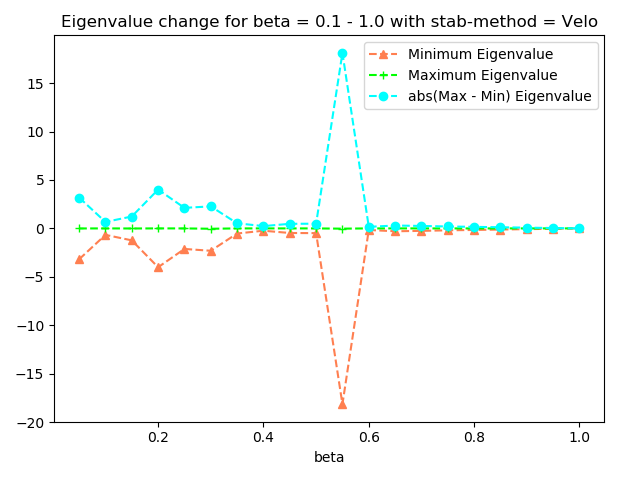
\includegraphics[width=0.8\textwidth]{Media/Beta_1_thru_0_velo.png}
    \end{center}
\end{frame}

\begin{frame}{Velocity Penalisation - Min Eigenvalue}
Velocity Penalisation:
      \(
      S = \beta\frac{\rho}{2}\bint \abs{\bmu \cdot \bmn }_- \bmu \cdot \bmv
      \)
    \begin{center}
        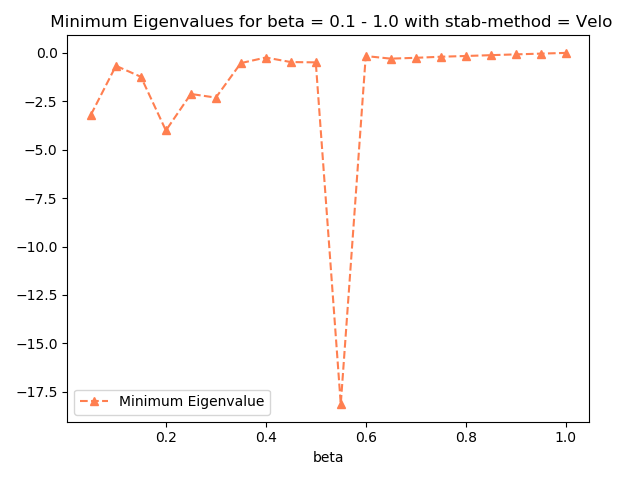
\includegraphics[width=0.8\textwidth]{Media/Beta_1_thru_0_velo_min.png}
    \end{center}
\end{frame}

\subsection{Tangential Penalisation Max}
% \begin{frame}{Change in eigenvalues over time}
%         \begin{center}
% \includemedia[
%     activate=onclick,
%     % activate=pageopen,
%     passcontext,
%     transparent,
%     width=0.75\textwidth,
% ]{
\includegraphics{Movies/cover.png}}{NoStabilisation.swf}
% \end{center}
% \end{frame}
\begin{frame}{Tang. Penalisation Max - Eigenvalues - Small Gamma}
Tang. Penal. Max: \(      S = \gamma U_b h^2 \frac{\rho}{2} \bint \qty(t^{T}\nabla\bmu \cdot t^{T}\nabla\bmv),  ~~U_b = \max \abs{\bmu \cdot \bmn}_-\)
    \begin{center}
        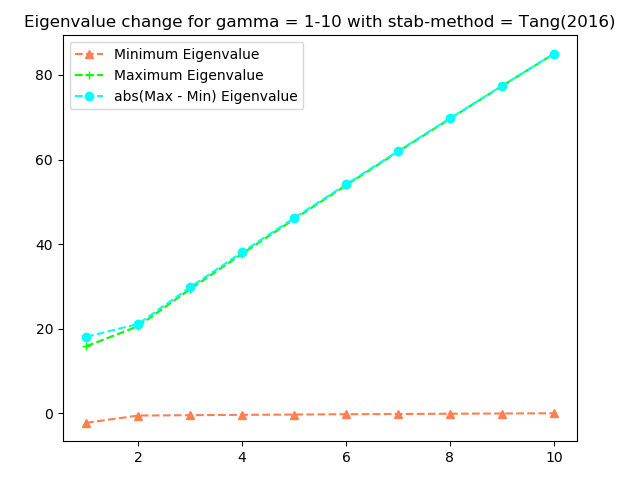
\includegraphics[width=0.8\textwidth]{Media/Gamma_1_thru_10_tang(2016).png}
    \end{center}
\end{frame}

\begin{frame}{Tang. Penalisation Max - Min Eigenvalues - Small Gamma}
Tang. Penal. Max: \(      S = \gamma U_b h^2 \frac{\rho}{2} \bint \qty(t^{T}\nabla\bmu \cdot t^{T}\nabla\bmv),  ~~U_b = \max \abs{\bmu \cdot \bmn}_-\)
    \begin{center}
        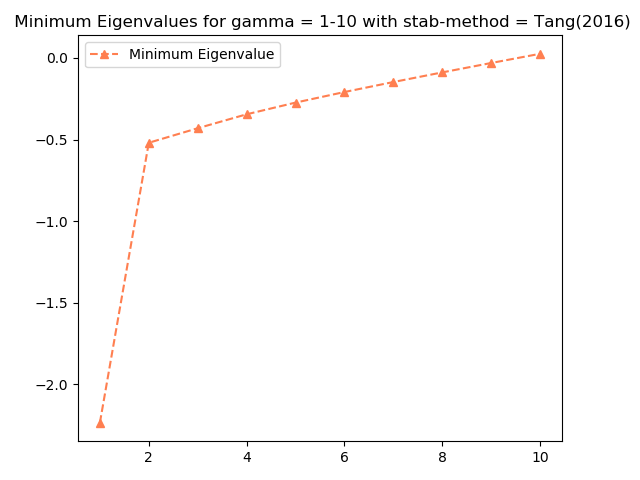
\includegraphics[width=0.8\textwidth]{Media/Gamma_1_thru_10_tang(2016)_min.png}
    \end{center}
\end{frame}

\begin{frame}{Tang. Penalisation Max - Eigenvalues - Large Gamma}
Tang. Penal. Max: \(      S = \gamma U_b h^2 \frac{\rho}{2} \bint \qty(t^{T}\nabla\bmu \cdot t^{T}\nabla\bmv),  ~~U_b = \max \abs{\bmu \cdot \bmn}_-\)
    \begin{center}
        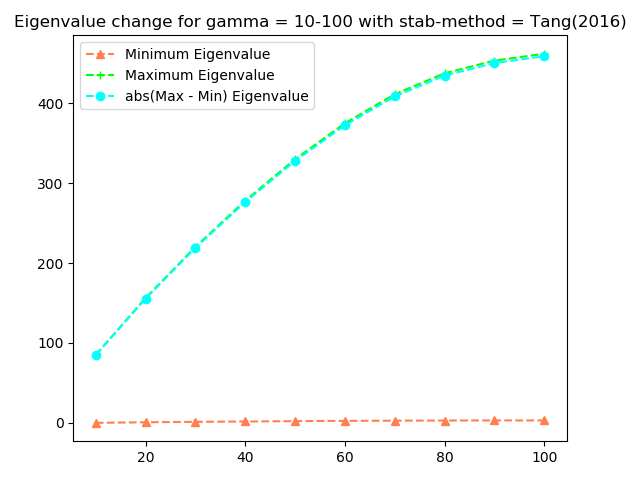
\includegraphics[width=0.8\textwidth]{Media/Gamma_10_thru_100_tang(2016).png}
    \end{center}
\end{frame}

\begin{frame}{Tang. Penalisation Max - Min Eigenvalues - Large Gamma}
Tang. Penal. Max: \(      S = \gamma U_b h^2 \frac{\rho}{2} \bint \qty(t^{T}\nabla\bmu \cdot t^{T}\nabla\bmv),  ~~U_b = \max \abs{\bmu \cdot \bmn}_-\)
    \begin{center}
        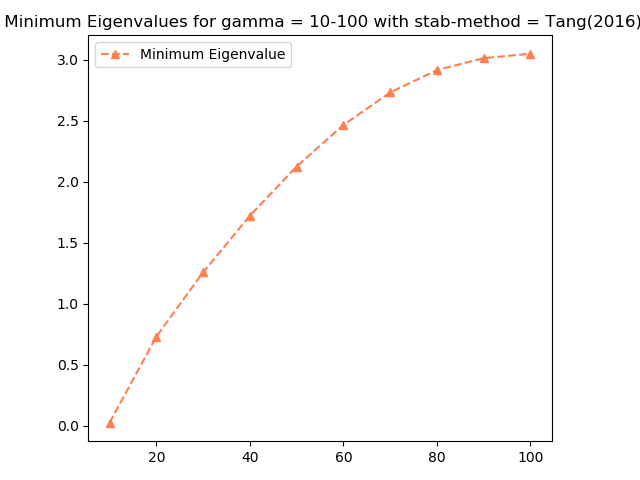
\includegraphics[width=0.8\textwidth]{Media/Gamma_10_thru_100_tang(2016)_min.png}
    \end{center}
\end{frame}

\begin{frame}{Tang. Penalisation Max - Test}
    \begin{center}
\includemedia[
    activate=onclick,
    % activate=pageopen,
    passcontext,
    transparent,
    width=0.75\textwidth,
]{
\includegraphics{Movies/cover.png}}{BFS4G100.swf}
\end{center}
\end{frame}

\subsection{Tangential Penalisation}
\begin{frame}{Tang. Penalisation - Eigenvalues - Small Gamma}
    Tang. Penalisation: \(
      S = \gamma\frac{\rho}{2}h^{2}\bint \abs{\bmu \cdot \bmn }_- \qty(t^{T}\nabla\bmu \cdot t^{T}\nabla\bmv)
      \)
    \begin{center}
        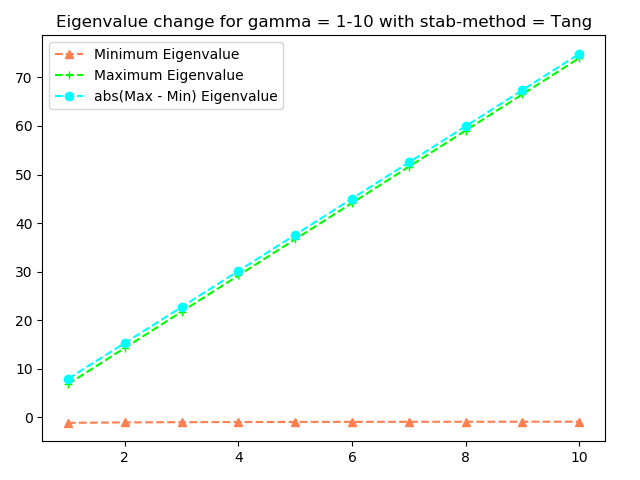
\includegraphics[width=0.8\textwidth]{Media/Gamma_1_thru_10_tang.png}
    \end{center}
\end{frame}

\begin{frame}{Tang. Penalisation - Min Eigenvalues - Small Gamma}
    Tang. Penalisation: \(
      S = \gamma\frac{\rho}{2}h^{2}\bint \abs{\bmu \cdot \bmn }_- \qty(t^{T}\nabla\bmu \cdot t^{T}\nabla\bmv)
      \)
    \begin{center}
        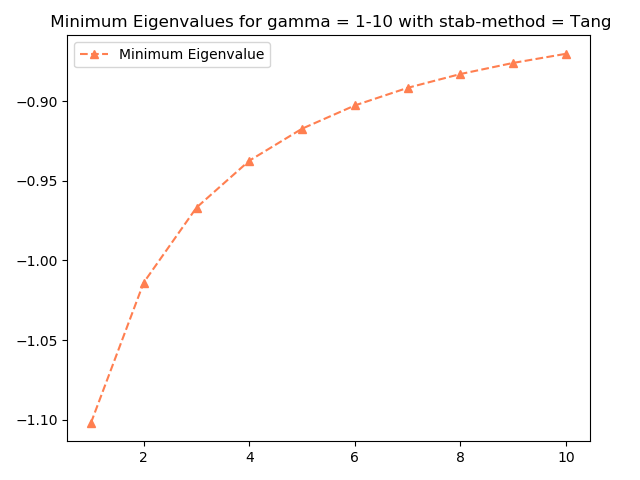
\includegraphics[width=0.8\textwidth]{Media/Gamma_1_thru_10_tang_min.png}
    \end{center}
\end{frame}

\begin{frame}{Tang. Penalisation - Eigenvalues - Large Gamma}
    Tang. Penalisation: \(
      S = \gamma\frac{\rho}{2}h^{2}\bint \abs{\bmu \cdot \bmn }_- \qty(t^{T}\nabla\bmu \cdot t^{T}\nabla\bmv)
      \)
    \begin{center}
        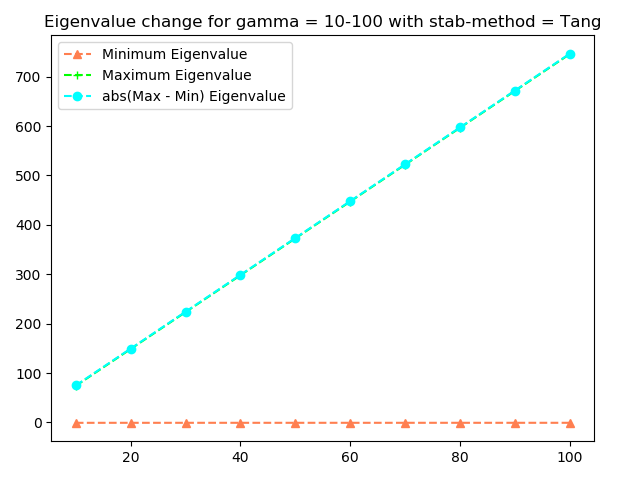
\includegraphics[width=0.8\textwidth]{Media/Gamma_10_thru_100_tang.png}
    \end{center}
\end{frame}

\begin{frame}{Tang. Penalisation - Min Eigenvalues - Large Gamma}
    Tang. Penalisation: \(
      S = \gamma\frac{\rho}{2}h^{2}\bint \abs{\bmu \cdot \bmn }_- \qty(t^{T}\nabla\bmu \cdot t^{T}\nabla\bmv)
      \)
    \begin{center}
        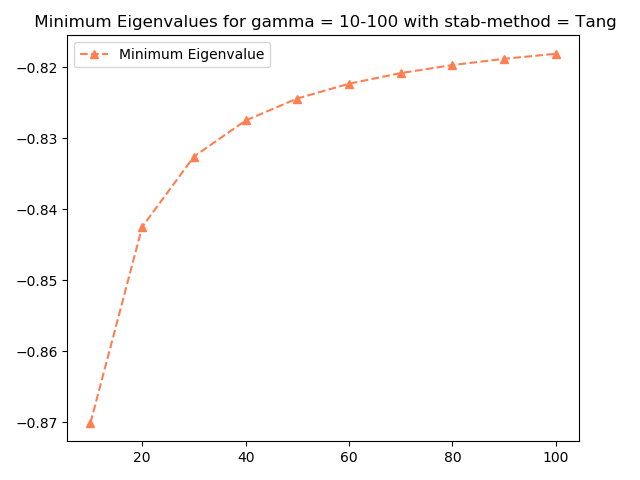
\includegraphics[width=0.8\textwidth]{Media/Gamma_10_thru_100_tang_min.png}
    \end{center}
\end{frame}

\begin{frame}{Tang. Penalisation - Test}
    \begin{center}
\includemedia[
    activate=onclick,
    % activate=pageopen,
    passcontext,
    transparent,
    width=0.75\textwidth,
]{
\includegraphics{Movies/cover.png}}{BFS3G100.swf}
\end{center}
\end{frame}